\documentclass[11pt, oneside]{article}   	% use "amsart" instead of "article" for AMSLaTeX format
\usepackage{geometry}                		% See geometry.pdf to learn the layout options. There are lots.
\geometry{letterpaper}                   		% ... or a4paper or a5paper or ... 
%\geometry{landscape}                		% Activate for rotated page geometry
%\usepackage[parfill]{parskip}    		% Activate to begin paragraphs with an empty line rather than an indent
\usepackage{amsmath}
\usepackage{amssymb}
\usepackage{amsfonts}
\usepackage{amsthm}
\usepackage[dvipdfmx]{graphicx}
% \graphicspath{{../figure/}}
\usepackage{mathtools}
\usepackage{algorithmic}
\usepackage{algorithm}
\usepackage{txfonts}
 \renewcommand{\algorithmicrequire}{\textbf{Input:}}
 \renewcommand{\algorithmicensure}{\textbf{Output:}}
 \newcommand{\argmax}{\mathop{\rm arg~max}\limits}
 \newcommand{\argmin}{\mathop{\rm arg~min}\limits}
 \usepackage[dvipdfmx]{graphicx}
 \newtheorem{thm}{Theorem}
\newtheorem{lem}[thm]{Lemma}
\newtheorem{axm}[thm]{Axiom}
\newtheorem{deff}[thm]{Definition}
\newtheorem{cor}[thm]{Corollary}
\newtheorem{prop}[thm]{Proposition}
\newtheorem{ass}{Assumption}
\newcommand{\diff}[1]{{\textcolor{red}{#1}}}
\usepackage{mathrsfs}
\usepackage{url}
%SetFonts

%SetFonts


\title{コンピュータ科学特別講義4 レポート課題2}
\author{コンピュータ科学専攻 修士課程1年 今村秀明 48-186112}
\date{}							% Activate to display a given date or no date

\begin{document}
\maketitle
\section{ソースコードについて}
%\subsection{}
まず、作成したプログラムのソースコードがあるgithubリポジトリは以下である。

\url{https://github.com/HideakiImamura/Parallel_Computing}

課題の作成に利用したソースコードは、ex2/src内にある。
各コードについて簡単に説明する。
まず、bitmap.cとbitmap.hは配布されたコードである。
また、img\_gen.cは実験用のサイズの大きなビットマップイメージを作成するためのコードである。
サイズが$60\times100$の画像が基本となり、これを$2^i\:\:(i = 0, 1, \ldots, 9)$倍に相似拡大した10枚の画像を生成する。
これらの画像は真っ黒な画像である。

そしてexperiment.cは実験を行うメインのコードである。
上で生成した10枚の画像それぞれに対して、スレッド数を1から8まで変化させて配布されたmain.cと同様の処理を行った。
スレッド数の最大値8は私の使用したPC であるMacBook Pro, 2.9GHz Intel Core i7の使用可能な最大プロセッサ数である。
csvファイルの形式で(使用スレッド数、画像の高さ、画像の幅、処理にかかった時間)を並べた物を出力した。

最後に、graph\_gen.pyはmatplotlibを用いて上で得られたcsvファイルをグラフ化するための補助的なコードである。

\section{スケーラビリティについて}
プログラムを実行して得られたグラフを以下に示す。
\begin{center}
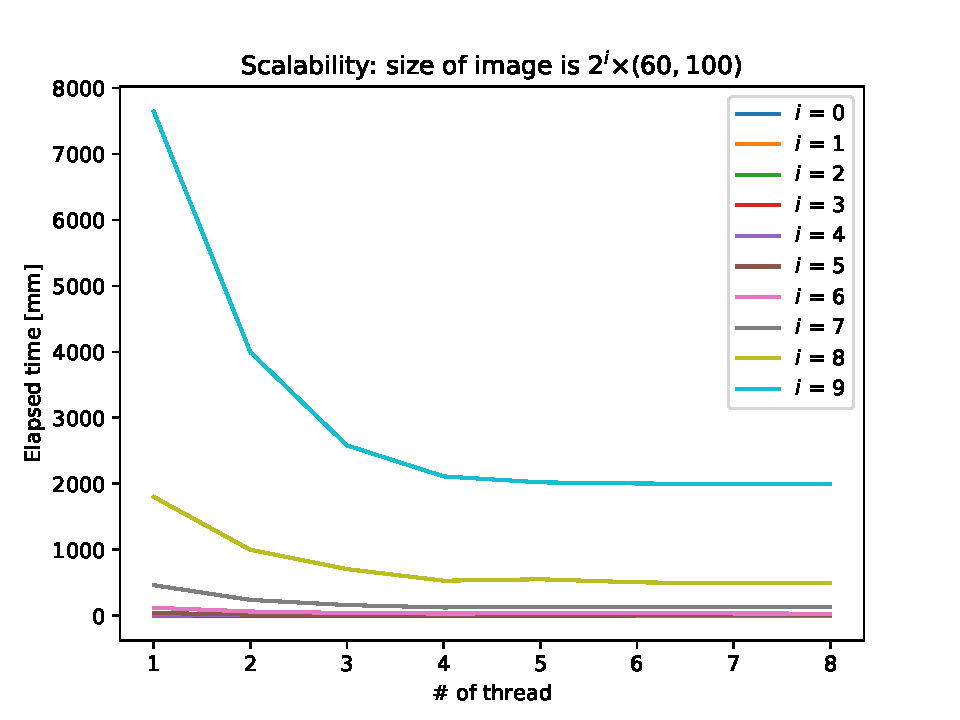
\includegraphics[width=10cm]{scalability.pdf}\\
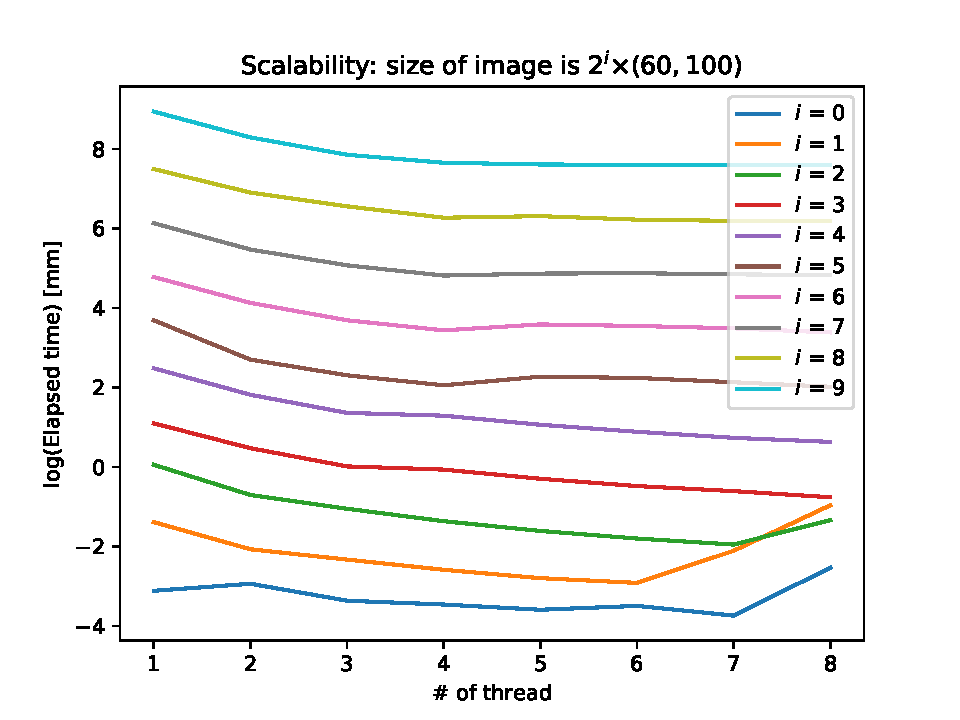
\includegraphics[width=10cm]{scalability_log.pdf}
\end{center}

各画像サイズごとにスレッド数に対する実行時間をプロットした。
上の画像では縦軸は実行時間をmmで示しており、下の画像では縦軸は実行時間の対数を取っている。
下の画像を見ればわかるように、画像サイズが$i=3$以上の段階で明らかな性能向上が見られる。
ただ、画像サイズが小さすぎる($i=0$や$i=1$)とスレッド数を増やしても性能が向上するとは限らないことが見て取れる。
これはスレッド数を増やしてもスレッド間の同期を取る時間といった本質的な並列処理以外の時間が大きくなるためだと考えられる。
また、上の画像を見ればわかるように、性能の向上はスレッド数に比例するわけではなく逓減していくことがわかる。
これはプログラム全体の中に並列可能な部分が一定の割合しかなく、アムダールの法則が成り立っていることを示唆している。

\section{アムダールの法則に基づく並列化可能な割合の計算}
アムダールの法則によれば、プログラム全体で並列化可能な部分の割合を$P$、その部分の性能向上率を$S$、全体の性能向上率を$A$とすると
\begin{align*}
	A = \frac{1}{(1 - P) + \frac{P}{S}}
\end{align*}
が成り立つ。
これを変形すると、
\begin{align*}
	P = \frac{\frac{1}{A} - 1}{\frac{1}{S} - 1}
\end{align*}
が得られる。
よって今、$S$を使用するスレッド数とし、$A$を実際の性能向上率とすると、$P$が計算できる。
$A$は具体的には以下のようにして計算する。
\begin{align*}
	A = \frac{\text{スレッド数が$1$の時の処理時間}}{\text{スレッド数が$S$の時の処理時間}}
\end{align*}
これを画像サイズを変化させて計算したグラフが以下である。
なお、$S$の値は8とした。
\begin{center}
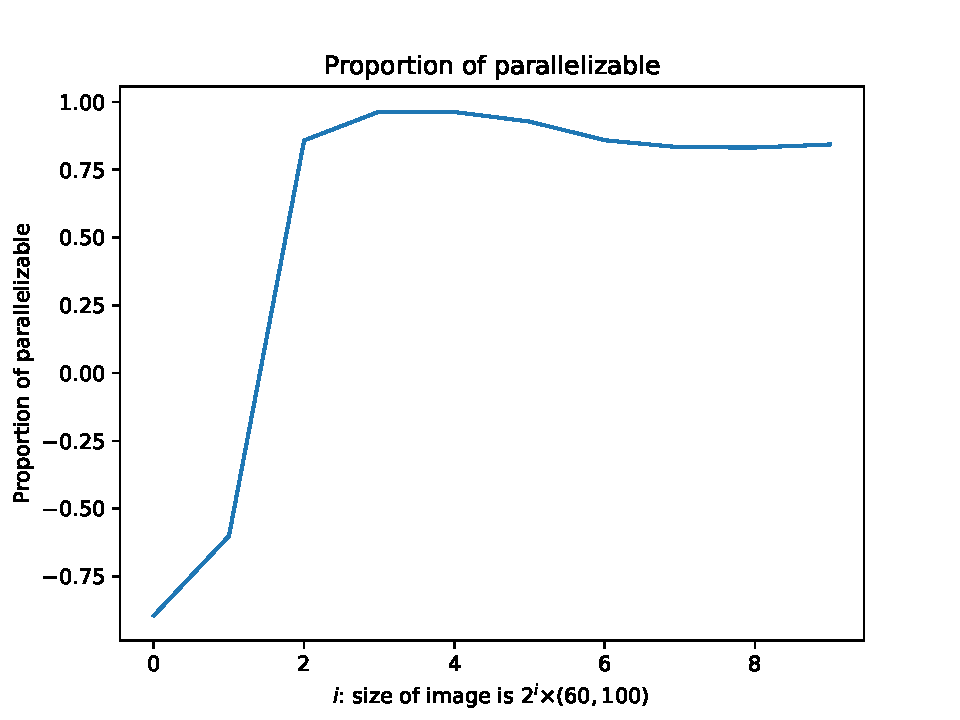
\includegraphics[width=10cm]{parallel.pdf}
\end{center}
このグラフから分かるように、画像サイズが大きくなるに従って$P$は大体$0.85$程度に収束していく。
画像サイズが小さい時は並列性を十分に利用できていないと考えられるから、画像サイズが大きい時に収束する0.85が、プログラム全体で並列化可能な割合であると考えられる。
\end{document}  